\section{Requirements}
\paragraph{} \textcite[4]{Sommerville.2000} define requirements as \say{a specification of what should be implemented}. \textcite[13]{Pohl.2007} clarifies the term, calling it a condition or a trait a person or a system must have to solve a problem or obtain a goal, as well as any condition or trait which is essential for fulfilling a contract, standard or specification, and any written documentation of those. Those definitions differ drastically. To understand the differences, one must understand the difference between requirement and specification that is done by \citeauthor{Pohl.2007}.
\paragraph{} Specification is defined by \textcite[220]{Pohl.2007} as being a special form of documentation of requirements that is done following a context specific set of rules. Thereby the definitions of specification - used by both authors - are on the one hand, technical specification in \citeauthor{Pohl.2007}'s work and targets for a systems in the work of \citeauthor{Sommerville.2000}. 
\paragraph{} in this thesis \citeauthor{Pohl.2007}'s definition of requirements will be applied, because it includes the documentation aspect of requirements and is more precise in terms of identifiable.
\subsection{Requirement Types \label{ssec:reqTypes}}
The types of requirements, appearing in most literature references, are functional and quality requirements. \textcite[14]{Lauesen.2008} says that \say{functional requirements specify the functions of the system, how it records, computes, transforms, and transmits data.} \textcite[cf.][15]{Pohl.2007} complements that functional requirements represent the functionality the aspired system shall provide its users. 
\paragraph{} In contrast to functional requirements, quality requirements describe the figure of merit of the desired product \parencite[cf.][15]{Lauesen.2008}. Quality requirements must be specifically measurable, because they otherwise cannot be verified \parencite[cf.][371-371]{Lauesen.2008}. For instance scales for quality can include performance, accuracy, availability, reliability etc. \parencite[cf.][15]{Pohl.2007}. \textcite[cf.][29]{Ebert.2014} adds an additional classification of quality requirements he specifies as external quality which includes the points mentioned above, and internal quality which reflects the qualification of the system for testing, maintenance, porting and so on. 
\paragraph{} \textcite[cf.][15]{Lauesen.2008} suggest that quality requirements are also called non-functional requirements. \textcite[cf.][16-17]{Pohl.2007} points out that this term is differently used across literature, and that most definitions just add unspecific functional requirements and quality requirements together. As an example, he shows the unspecific functional requirement shown in \Cref{tab:reqSpec} (a) which cannot concern the quality due to the lack of measurability. Thereby it can only be a functional requirement. \textcite[17]{Pohl.2007} shows an exemplary specification of a  functional requirement in \Cref{tab:reqSpec} (b) to (e).

\begin{table}[H]
    \centering
    \begin{tabular}{|c|c|m{10cm}|}
        \hline
        (a) & R1 & The system  must be secure.\\
         \hline
        \hline
        (b) & R1.1 & The user must authenticate to gain access to the system.\\
        \hline
        (c) & R1.2 & The authentication of the user must be done by using a digital certificate.\\
        \hline
        (d) & R1.3 & All data exchange between the user client and the system server must be encrypted.\\
        \hline
        (e) & R1.4 & Encryption of communication via an insecure network must be using a asynchronous encryption method with a key length of at least 1024 bit.\\
        \hline
    \end{tabular}
    \caption[Specification of unspecific Functional Requirement]{Specification of unspecific Functional Requirement \parencite[17]{Pohl.2007}}
    \label{tab:reqSpec}
\end{table}

\paragraph{} In this thesis, the term non-functional requirement will not find any more appliance, in order to reduce the risk of confusion, misunderstanding and mislabeling.
\paragraph{} \textcite[29]{Ebert.2014} and \textcite[18-19]{Pohl.2007} agree upon a third category of requirements, which are specified as not being easy to be changed. These requirements are called constraints and are preset conditions. Examples for constraints are legal limitations, financial budgets, maximum development time and so on. In comparison, constraints are not functional nor quality requirements. That is to say, they restrict those by prohibition or by limitation of resources in a way, that prioritization is the imperative.
\paragraph{} The types of categories, not having shown overlapping definitions in the literature, are used in this paper and can be seen in \Cref{fig:reqTypes}.

\begin{figure}[H]
    \centering
    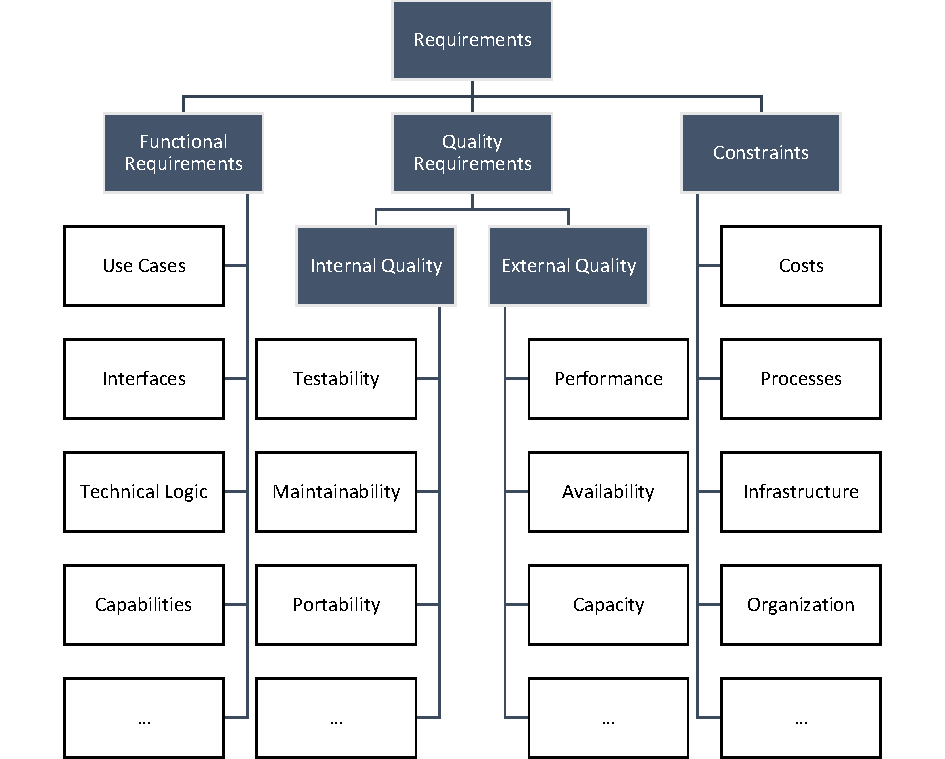
\includegraphics[scale=1]{img/RequirementTypes.pdf}
    \caption[Requirement Types]{Tpes of Requirements used in this paper (own illustration)}
    \label{fig:reqTypes}
\end{figure}
\subsection{Requirements Engineering \label{ssec:reqEn}}
Engineering requirements for a to-be system requires a diverse set of input information (cf. \Cref{fig:reqFlow}). The goal of requirement engineering is to produce a set of requirements fitting to a modeled and specified system \parencite[cf.][28]{Kotonya.2000}. A repetitive\label{iterative} and systematic approach to generate complete, relevant, consistent etc. requirements is implied by the term of requirement engineering \parencite[5]{Sommerville.2000}, including sourcing and management of requirements \parencite[262]{Pohl.2007}.
\begin{figure}[H]
    \centering
    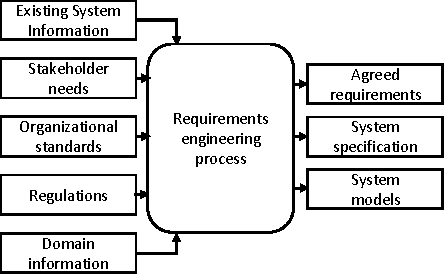
\includegraphics[scale=1.3]{img/RequirementInformationStream.pdf}
    \caption[Information flow in Requirements Engineering]{Information flow in Requirement Engineering (\protect\cite[28]{Kotonya.2000})}
    \label{fig:reqFlow}
\end{figure}
Information sources for Requirements Engineering include:
\begin{enumerate}
    \item Not only, legacy systems are sources for existing system information if applicable, but also systems to be interacted with \parencite[cf.][28]{Kotonya.2000}.
    \item Stakeholders of a system are people or institutions that have some kind of direct or indirect causal relation with the system \parencite[cf.][8]{Sommerville.2000}. This may be users, developers, sponsors, customers, employees and many more. Each stakeholder has some needs for the system - being motivated by political interests in the organization, support of work, legal determinations or something different \parencites[cf.][28]{Kotonya.2000}[cf.][350-351]{Lauesen.2008}
    \item Organizational standards enforce conformaty assurance within one company by regulating system development, quality management etc. \parencite[28]{Kotonya.2000}
    \item Regulations seek to protect the interests of certain stakeholders, e.g. health and safety regulations \parencite[cf.][28]{Kotonya.2000}.
    \item \say{Domain information [..] about the application domain of the system} \parencite[28]{Kotonya.2000} 
\end{enumerate}

\subsubsection{Requirement Engineering Process:} The\say{Requirements Engineering Framework} by \textcite{Pohl.2007} defines a systemic approach to fill the gap between input information and the vision and goals of a desired output (cf. \Cref{fig:reqFramework}). It analyzes the input information into four different facet of the system context: entities, IT-system, usage and development of the desired application. Information is processed in three main activities\label{mainactivity} (documentation, sourcing and confirmation) and two cross-sectional activities (validation and management), which lead to the requirement artifacts which represent the vision and goals of the product. \parencite[cf.][38-39]{Pohl.2007}
\begin{figure}[H]
    \centering
    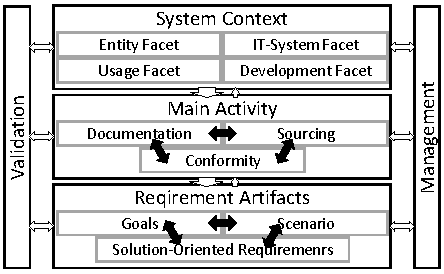
\includegraphics[scale=1.5]{img/ReqAnFrameWork.pdf}
    \caption[Framework for Requirements Engineering]{Framework for Requirements Engineering (own illustration based on \cite[41]{Pohl.2007})}
    \label{fig:reqFramework}
\end{figure}
\subparagraph{} \label{beginFacets} Defining the boundary of system context is essential for successful requirements engineering. It reflects in what way the desired outcome is related entities of whatever kind \parencite[55]{Pohl.2007}. Context diagrams \parencites[cf.][266]{Kossiakoff.2011} - as an example for visual system context representation - treat the system \say{as a black box surrounded by user groups and external systems with which it communicates} \parencite[76]{Lauesen.2008}. The system context represents the environment of a system, which is relevant for requirement analysis \parencite[55]{Pohl.2007}. System context boundary definitions must be formulated to scope out the not relevant part of the system environment \parencite[55-56]{Pohl.2007}. The four facets for structuring input information of the system context of \textcite{Pohl.2007} are the following:
\begin{enumerate}
    \item Entities are the digital representation of real world objects and their traits. This can include people such as users and subjects, physical objects such as assets, immaterial objects such as measurements, and processes. Important stakeholders are  professionals for the technical view and legal advisor and data security officials ensuring compliance. \parencite[cf.][70-71]{Pohl.2007}
    \item The facet of the IT-system in the system context is considering interface requirements to other technical systems such as the underlying hardware or systems the desired product must or may interchange data with \parencite[cf.][192]{Kotonya.2000}. Relevant stakeholders are architects, developers, and test and maintenance professionals of the context systems \parencite[cf.][72]{Pohl.2007}.
    \item The usage facet deals with the demand by direct and indirect users for the system. User in this context are people and systems having a direct interface with the desired product or are somehow impacting the interaction with the desired product or are impacted by usage of the system. \parencite[cf.][75-77]{Pohl.2007}
    \item All information about the development process is regarded by the development facet. Stakeholders and sources for this facet predominantly are people involved with the design, implementation and controlling of the development process, guidelines, standards and norms for development, and best practices and project reports. \parencite[cf.][79]{Pohl.2007}
\end{enumerate}
\label{endFacet}
\begin{figure}[H]
    \centering
    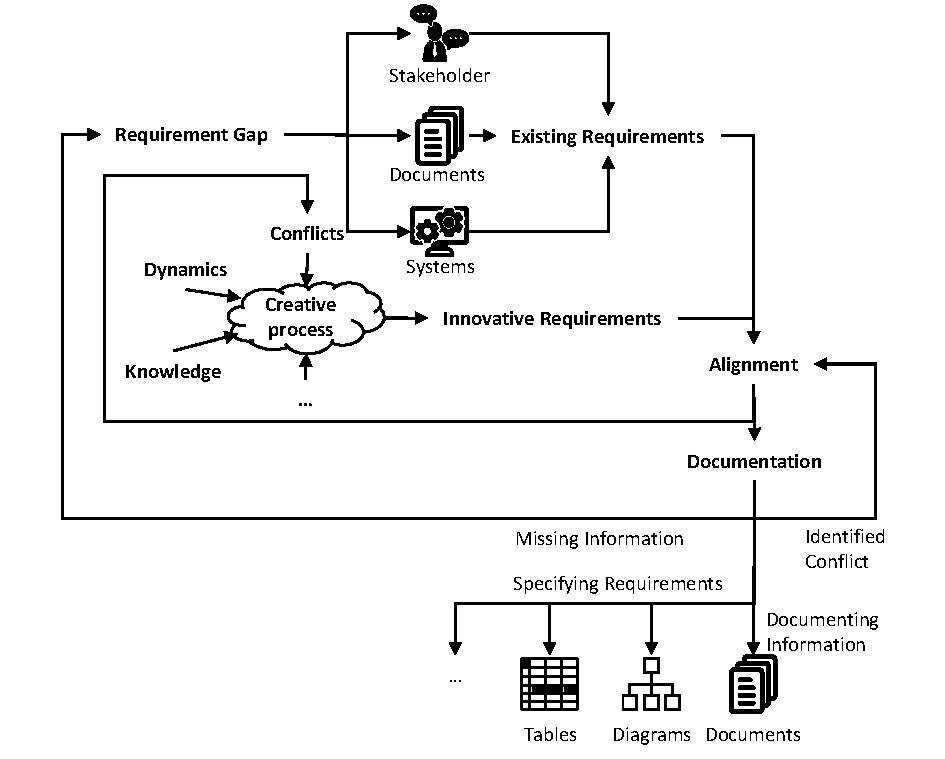
\includegraphics[scale=1]{img/MainActivity.pdf}
    \caption[Information Flow in Main Activity of Requirements Engineering]{Information Flow in Main Activity  (own illustration)}
    \label{fig:infFlow}
\end{figure}
\subparagraph{}\label{beginmain} The main activities are interlinked by continuously exchanging information. \Cref{fig:infFlow} sows a minimalist outline of that flow of information. Starting from the supplied information by stakeholders, documents, etc. requirements are generated, aligned for conformity, and specified and documented. Feedback loops resolve occurring errors such as conflicts of requirements or gaps.
\begin{enumerate}
    \item Sourcing requirements founds on two different goals: detecting existing requirements, and create innovative requirements \parencite[cf.][318, 321]{Pohl.2007}. This is done by taking information from the information sources (see \Cref{fig:reqFlow}) and analyzing the underlying needs \parencite[cf.][75-76]{Sommerville.2000}. Whenever conflicts of requirements, group dynamics etc. generate demand for an additional requirement without specific needs or a trade-off solution, a creative approach can be used to innovate new requirements \parencite[cf.][94]{Lauesen.2008}. 
    \item The conformity activity seeks and identifies competing requirements - in content, limited resources, or priority - in order to resolve those issues. The Conformity activity seeks to resolve those issues by analysis and management of conflicts. Possible solutions include management decisions, trade-offs, or inducing change requests. \parencite[cf.][393]{Pohl.2007}
    \item{Documentation} is used for recording all relevant information gathered in the main and cross-section activities \parencite[cf.][217]{Pohl.2007}. Requirements Engineering distinguish two subsets of documented information: documented requirements and specified requirements. Only requirements that have been parsed from informal descriptions - as they are most commonly provided by operational or marketing departments - into standardized requirement templates are specified requirements \parencite[cf.][101]{Ebert.2014}. Depending on the kind of information to be documented, different levels of specification are necessary. The documenting activity helps to identify gaps and conflicts in existing requirements giving input to the other main activities \parencite[212]{Pohl.2007}\label{endmain}
\end{enumerate}

\subparagraph{} Requirement artifacts are documented requirements \parencite[85]{Pohl.2007}. There are three complementary categories of requirement artifacts: 

\begin{enumerate}
    \item Intentions of the stakeholders are documented as goals \parencite[cf.][85]{Pohl.2007}, substanciating the product vision \parencite[cf.][54]{Ebert.2014}. Goals are decomposed into groups of subgoals connected by logical AND and OR gateways \parencite[cf][91]{Pohl.2007}. Goal level requirements are optimal for understanding the reason for requirements, because they reflect the value of the requirement to the stakeholder \parencite[cf.][25]{Lauesen.2008}.
    \item Scenarios are list of steps in the system context that need to be done to fulfill a goal level requirement \parencite[125]{Pohl.2007}. \say{A scenario is an instantiation of a use case} \parencite[114]{Lauesen.2008}, meaning that each scenario matches a process within the system, or interaction with the system, including a desired outcome \parencite[cf.][114]{Lauesen.2008}.
    \item Deducing from goals and scenarios, solution-oriented requirements specify all relevant information for developing the desired application \parencite[cf.][182-184]{Pohl.2007}. These requirements are based on three different perspectives (data, functionality and behaviour) and are documented in natural language and/or in models \parencite[cf.][184-187]{Pohl.2007}. Commonly sentence patterns are used for natural language documentation      
\end{enumerate}

\subparagraph{} Cross-Sectional Activities are done within each segment of requirements engineering \parencite[cf.][417, 493]{Pohl.2007}. 
Validating the results of predefined process steps reduces the costs of changes done as the requirement engineering progresses \parencite[cf.][419]{Pohl.2007}. For that reason a set of quality specifications for intermediate and final results must be defined in advance of the engineering phase \parencite[cf.][418]{Pohl.2007}.
The Management activity continuously watches and - if necessary - adjusts the definition of the system context, coordinates the main activities and organizes the requirement artifacts. \parencite[cf.][493]{Podjarny.2014}.